\documentclass[a4paper]{article}

\usepackage[
    fontset=none,%设置中文支持,并自定义字体
    zihao=5,%默认字号为五号
    heading=true,%允许后续自定义标题样式
    scheme=chinese,%自动将文档样式中文化,例如图标标题
    punct=quanjiao,%全角式标点符号
    space=auto,%中文后接换行不会添加空格,但是英文会添加空格,需要用%手动取消
    linespread=1.3,%行距倍数是1.3
    autoindent=true,%自动缩进两个中文宽度
    ]{ctex}
\ctexset{
    % tday=small,%小写样式的日期
    contentsname={目录},
    listfigurename={插图},
    listtablename={表格},
    figurename={图},
    tablename={表},
    abstractname={摘要},
    indexname={索引},
    appendixname={附录},
    bibname={参考文献},
    proofname={证明},
    % refname={参考文献},%只适用于beamer
    % algorithmname={算法},
    % continuation={(续)},%beamer续页的标识
    section={
        format+ = \Large\heiti\raggedright,
        name = {,\num\textbf{.}\hspace{1ex}},
        number={\num\thesection},
        nameformat={},
        numberformat={},
        aftername={},
        titleformat={},
        aftertitle={},
        runin=false,%对section级以下有用,标题是否和正文在同一段上
        beforeskip={3.5ex plus 1ex minus .2ex},%标题前垂直间距
        afterskip={2.3ex plus .2ex}%标题后垂直间距
    },
    subsection={
        format+ = \large\heiti\raggedright,
        name = {,\num\textbf{.}\hspace{1ex}},
        number={\num\thesubsection},
        nameformat={},
        numberformat={},
        aftername={},
        titleformat={},
        aftertitle={},
        runin=false,%对section级以下有用,标题是否和正文在同一段上
        beforeskip={3.5ex plus 1ex minus .2ex},%标题前垂直间距
        afterskip={2.3ex plus .2ex}%标题后垂直间距
    },
    subsubsection={
        format+ = \normalsize\heiti\raggedright,
        name = {,\num\textbf{.}\hspace{1ex}},
        number={\num\thesubsubsection},
        nameformat={},
        numberformat={},
        aftername={},
        titleformat={},
        aftertitle={},
        runin=false,%对section级以下有用,标题是否和正文在同一段上
        beforeskip={3.5ex plus 1ex minus .2ex},%标题前垂直间距
        afterskip={2.3ex plus .2ex}%标题后垂直间距
    },
    }

% 中文默认字体: 思源宋体,粗体为思源宋体半粗体,斜体为方正楷体_GBK
\setCJKmainfont{Source Han Serif SC}[BoldFont={Source Han Serif SC Heavy}, ItalicFont=FZKai-Z03S]
% 中文无衬线字体:思源黑体,粗体为思源黑体粗体
\setCJKsansfont{Source Han Sans CN}[BoldFont={Source Han Sans CN Heavy}]
% 中文等宽字体:微软雅黑light
\setCJKmonofont{Microsoft YaHei}[ItalicFont={Microsoft YaHei Light}]

\newCJKfontfamily\songti{Source Han Serif SC}[BoldFont={Source Han Serif SC Heavy}]
\newCJKfontfamily\xbsong{Source Han Serif SC SemiBold} % 小标宋
\newCJKfontfamily\dbsong{Source Han Serif SC Bold} % 大标宋
\newCJKfontfamily\cusong{Source Han Serif SC Heavy} % 粗宋
\newCJKfontfamily\heiti{Source Han Sans CN}[BoldFont={Source Han Sans CN Heavy}]
\newCJKfontfamily\dahei{Source Han Sans CN Medium} % 大黑
\newCJKfontfamily\cuhei{Source Han Sans CN Heavy} % 粗黑
\newCJKfontfamily\fangsong{FZFangSong-Z02S}
\newCJKfontfamily\kaiti{FZKai-Z03S}[ItalicFont={Microsoft YaHei Light}]%这个斜体只是用于lstlisting环境中的中文注释
% \newCJKfontfamily\kaiti{FZKai-Z03S}[ItalicFont={FZZJ-LZXTFSJW}]%这个斜体只是用于lstlisting环境中的中文注释
\setsansfont{Arial}
\setmonofont{Consolas}%设置西文等宽字体
\newfontfamily\code{Consolas}
\newfontfamily\num{Arial}

\usepackage{geometry}%设置整体页面布局
\geometry{a4paper}
\geometry{left=2cm,right=2cm,top=2.54cm,bottom=2.54cm}%word常规页边距
% \geometry{left=1.27cm,right=1.27cm,top=1.27cm,bottom=1.27cm}%word窄页边距
\setlength{\headheight}{13pt}%避免warning


\usepackage{fancyhdr}%必须在geometry包之后使用
\fancyhf{}
\makeatletter
\lhead{{\dahei \@title}}%可以使用thepage,CTEXthechapter,CTEXthesection
\makeatother
\rhead{\textbf{\num- \thepage{} -}}
\renewcommand\headrulewidth{1.5pt}%设置眉头宽度
\pagestyle{fancy}

\usepackage[ruled,algosection,lined,longend,fillcomment,linesnumbered,resetcount,titlenotnumbered]{algorithm2e}
%参数解释:带框,按section编码,有竖线,end前带if等关键词,注释占满整行,代码部分编号(不包括输入输出、注释),每个代码块重新编号,可以调用TitleOfAlgo来打印算法标题但不作为单独的算法编码
%附带algorithm,function,procedure环境,其中function,procedure环境下,设置caption时,必须带有(),
%()之前的字符会被视为宏,可以在接下来的部分用\名字()来调用,所以推荐辅助函数用function,其中的某些展开部分用procedure,描述算法整体使用algorithm
\DontPrintSemicolon
\SetAlCapSkip{2ex}
\SetSideCommentRight
\SetFillComment
\newcommand{\forcond}{$i=0$ \KwTo $n$}
\SetKw{downto}{downto}%自定义关键词
\SetKwFunction{funcmacro}{text}%自定义函数名,实际上function环境是在定义宏的同时说明了其内容
\SetKwProg{procedmacro}{text}{begin text}{end text}%自定义步骤,和function类似,但是后面两个参数可以设置开始和结尾的标志,和if等环境一样
\SetKwData{datamacro}{text}%可以用于突出特殊的变量,例如数据结构
\SetKwFunction{FRecurs}{FnRecursive}
\SetKwProg{Fn}{Function}{begin}{end}

\usepackage[strict]{changepage}
\usepackage{framed}%色块支持
\definecolor{formalshade}{rgb}{0.95,0.95,1} % 文本框颜色
% ------------------******-------------------
% 注意行末需要把空格注释掉,不然画出来的方框会有空白竖线
\newenvironment{formal}{%
\def\FrameCommand{%
\hspace{1pt}%
{\color{DarkBlue}\vrule width 2pt}%
{\color{formalshade}\vrule width 4pt}%
\colorbox{formalshade}%
}%
\MakeFramed{\advance\hsize-\width\FrameRestore}%
\noindent\hspace{-4.55pt}% disable indenting first paragraph
\begin{adjustwidth}{}{7pt}%
\vspace{2pt}\vspace{2pt}%
}
{%
\vspace{2pt}\end{adjustwidth}\endMakeFramed%
}

% 自定义标题格式
\makeatletter
\renewcommand{\maketitle}{
  \begin{center}
    \thispagestyle{fancy}
    {\quad}\\
    \vspace{0.1\textheight}
    {\huge\sffamily\bfseries\@title}\\ % 标题字体大小、粗体、颜色
    \vspace{2em} % 标题与作者名之间的垂直空间
    {\large\sffamily\@author} \\
  \end{center}
}
\makeatother

\usepackage{graphicx}

\title{作业{\hspace{1ex}}HW4}
\author{姓名:范潇{\quad}学号:2254298{\quad}日期:\today}
\date{}
\begin{document}
\maketitle
\section{7.1}
记分解得到的两个关系分别为$R_1,R_2$,则$R_1\cap R_2=A$,因为
\[A\rightarrow BC\]
\[A\rightarrow A\]
所以有
\[A\rightarrow R_1\]
即
\[R_1\cap R_2\rightarrow R_1\]
所以是无损分解。
\section{7.6}
$F^{+}$可以通过枚举所有的$\bm{\alpha}$,计算出$\bm{\alpha}^{+}$,然后将形如$\bm{\alpha}\rightarrow\bm{\beta},\bm{\beta}\subseteq \bm{\alpha}^{+}$的函数依赖添加入$F^+$即可。

$X=\varnothing,Y=\{A,B,C,D,E\},$

第一轮: 

$A^+=R,B^+=\{B,D\},C^+=\varnothing,D^+=\varnothing,E^{+}=R$,所以$A$和$E$为候选码.

第二轮:

$BC^+=R,BD^+=\{B,D\},CD^+=R$,所以$BC$和$CD$为候选码。

综上,候选码有$A,E,BC,CD$.
% 第一轮:

% 使用自反律推得函数依赖
% \[A\rightarrow\varnothing,A\rightarrow A\]
% \[CD\rightarrow\varnothing,CD\rightarrow C,CD\rightarrow D\]
% \[B\rightarrow\varnothing,B\rightarrow B\]
% \[E\rightarrow\varnothing,E\rightarrow E\]
% 使用增广律推得函数依赖
% \[A\rightarrow ABC,AB\rightarrow BC,AC\rightarrow BC,AD\rightarrow BCD,AE\rightarrow BCE\]
% \[ACD\rightarrow AE,BCD\rightarrow BE,CD\rightarrow CE,CD\rightarrow DE,CDE\rightarrow E\]
% \[AB\rightarrow AD,B\rightarrow BD,BC\rightarrow CD,BD\rightarrow D,BE\rightarrow DE\]
% \[AE\rightarrow A,BE\rightarrow AB,CE\rightarrow AC,DE\rightarrow AD,E\rightarrow AE\]
% 使用传递律推得函数依赖
% \[AC\rightarrow CD\]
% \[AD\rightarrow BE\]
% \[BCD\rightarrow DE\]
% \[CD\rightarrow AC\]
% \[CDE\rightarrow AE\]
% \[B\rightarrow D\]
% \[AE\rightarrow ABC\]
% \[BE\rightarrow BC,BE\rightarrow AD\]
% \[CE\rightarrow BC\]
% \[DE\rightarrow BCD\]
% \[E\rightarrow BCE,E\rightarrow A\]
\section{7.30(a,b,c,d)}
\begin{enumerate}
    \item $B^+=\{A,B,C,D,E\}$
    \item 因为 $BC\rightarrow DE$,由增广律可得$ABCD\rightarrow ABCDE$。又因为$A\rightarrow BCD$,由增广律可得$A\rightarrow ABCD$。从而由
    传递律可得$A\rightarrow ABCDE$,再由增广律可得$AG\rightarrow ABCDEG$,从而$AG$为超码。
    \item 一个正则覆盖为 $\{A\rightarrow BC,BC\rightarrow E,B\rightarrow D,D\rightarrow A\}$,这是通过把$A\rightarrow BCD$改为$A\rightarrow BC$,把 
    $BC\rightarrow DE$改为$BC\rightarrow E$得到的。因为$A\rightarrow BC,B\rightarrow D$能够推出$A\rightarrow BCD$,同时$BC\rightarrow E$和$B\rightarrow D$能够推出$BC\rightarrow DE$.
    \item 一个第三范式分解为$(ABC,BCE,BD,AD,AG)$,其中只有$AG$包含候选码。
\end{enumerate}
\section{Quiz}
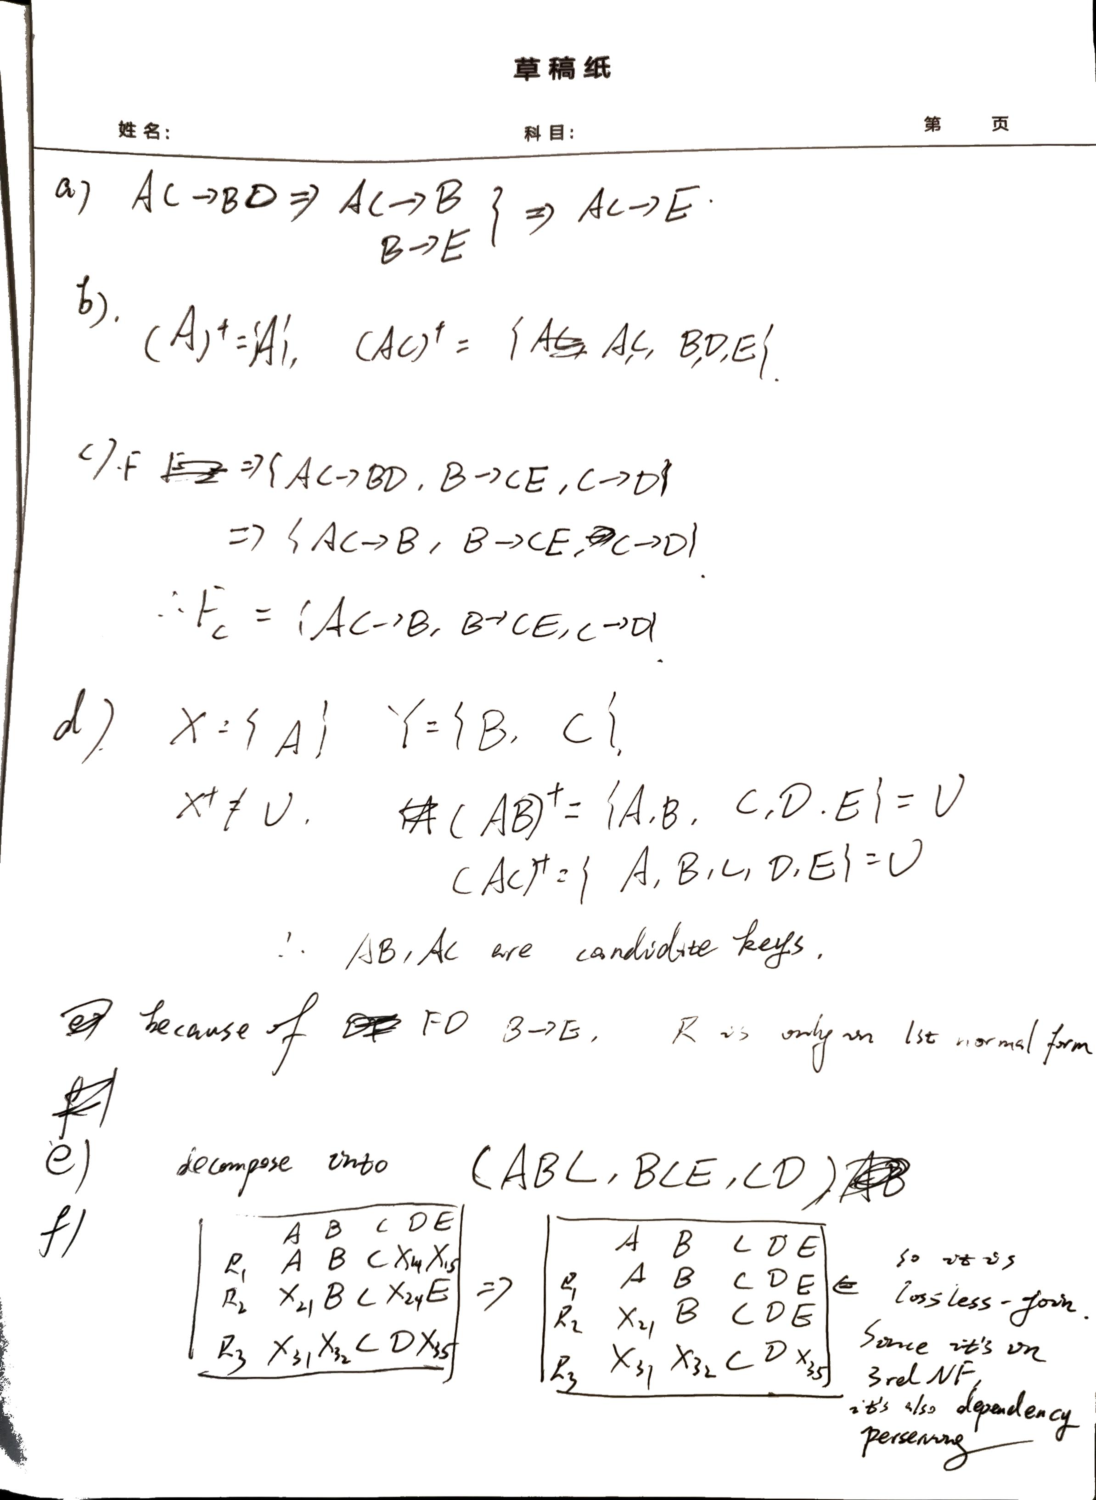
\includegraphics[width=\textwidth]{quiz.pdf}
\end{document}